\documentclass[12pt]{article}


\usepackage[spanish]{babel}
\usepackage[utf8]{inputenc}
\usepackage[T1]{fontenc}

%paquetes matematicos
\usepackage{amsmath, amsfonts, amssymb}

%dimensiones
\usepackage[left=2.5cm, right=2.5cm, top=2cm]{geometry}

%para las imagenes y mas...
\usepackage{graphicx}
\usepackage{subfig}
\graphicspath{ {imagenes/} }
\usepackage{float}

\title{Equivalencia entre Expresiones Regulares y Autómatas}
\author{Ian Mendoza Jaimes}
\date{}

\begin{document}
\maketitle
\begin{center}
2CM4

Profesor: Genaro Juárez Martínez

16 de octubre de 2016
\end{center}

\vspace{3em}

Las expresiones regulares son otro tipo de notación para definir un lenguaje \textit{L}. Estas expresiones están íntimamente relacionadas con los Autómatas Finitos no Determinísticos y pueden ser pensadas también como una manera un tanto más amigable para describir algunos componentes de un software. \\

En este ejemplo se a pedido construir el autómata que describe al mismo lenguaje que la siguiente expresión regular \textit{E}: 
\[E=(0+1)^{*}01\]
Primero se encontró el autómata finito no determínistico, el cual es el siguiente:

\begin{figure}[H]
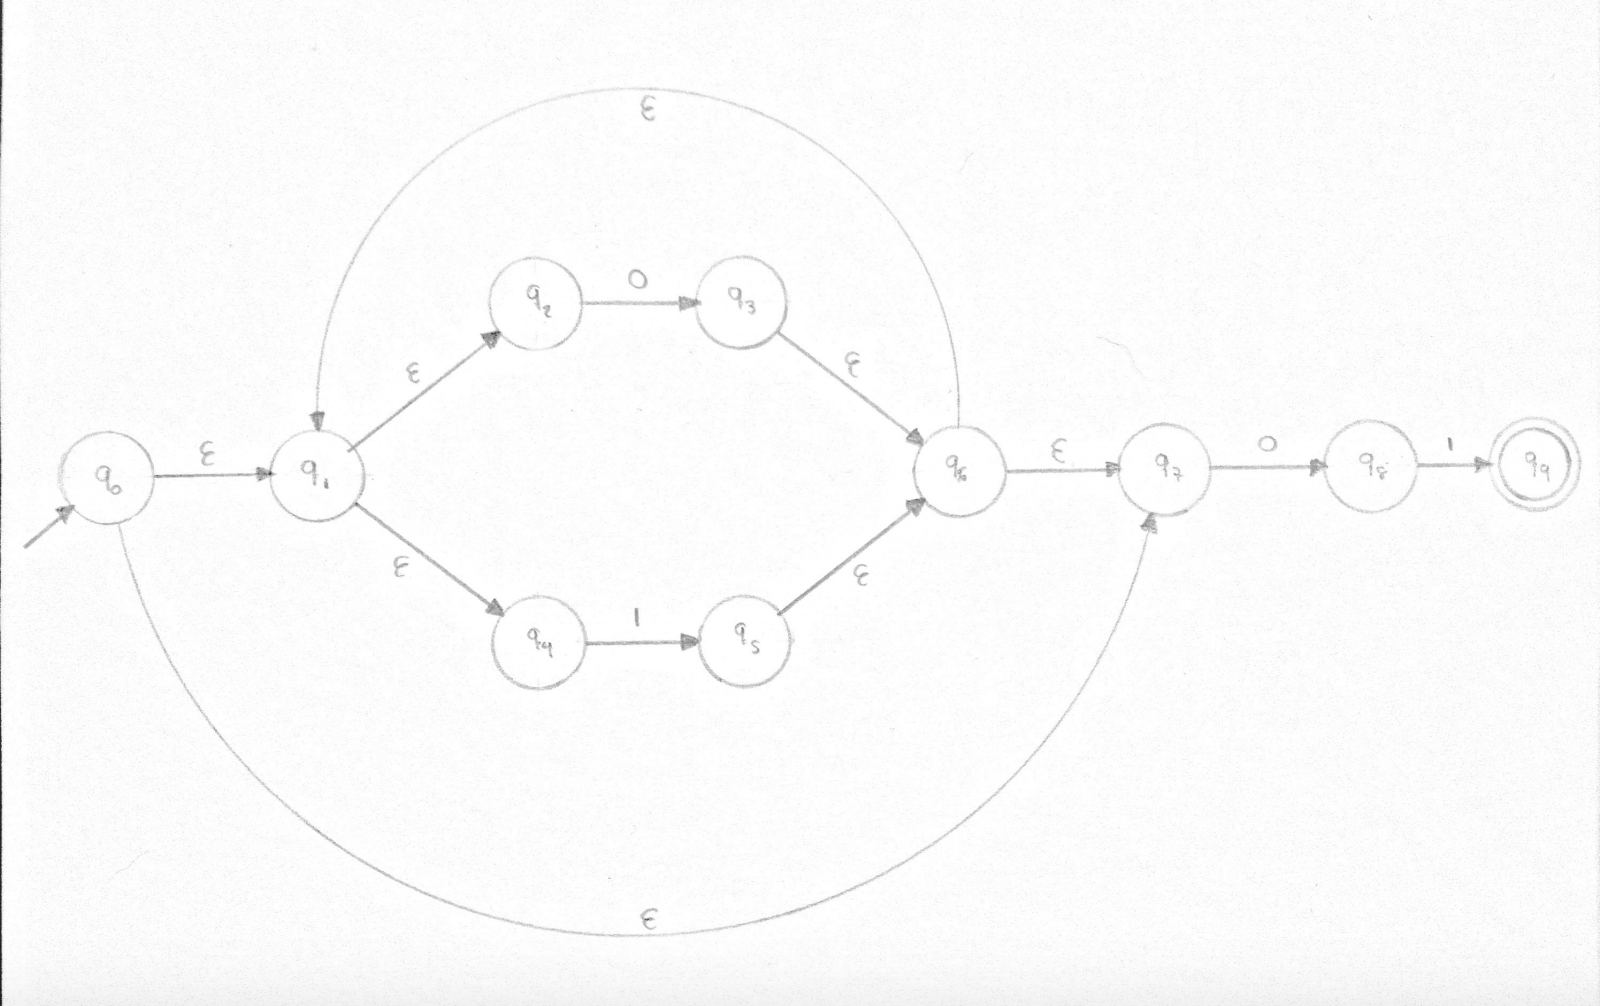
\includegraphics[width=\textwidth, height=9cm]{nfa}
\caption{Conversión de \textit{E} a un \textit{NFA}.}
\end{figure}

Formalmente el anterior es un $\epsilon-NFA$, y la tabla que se obtuvo para transformarlo a un \textit{DFA} es la siguiente: \\

\begin{table}[H]
\centering
\begin{tabular}{|c|c|c|}
\hline 
 & 0 & 1 \\ 
\hline 
$\rightarrow\lbrace$ q0,q1,q2,q4,q7 $\rbrace$ & $\lbrace$ q3,q6,q7,q1,q2,q4,q8 $\rbrace$ & $\lbrace$ q5,q6,q7,q1,q2,q4 $\rbrace$ \\ 
\hline 
$\lbrace$ q3,q6,q7,q1,q2,q4,q8 $\rbrace$ & $\lbrace$ q8,q3,q6,q7,q1,q2,q4 $\rbrace$ & $*\lbrace$ q5,q6,q7,q1,q2,q4,q9 $\rbrace$ \\ 
\hline 
$\lbrace$ q5,q6,q7,q1,q2,q4 $\rbrace$ & $\lbrace$ q8,q3,q6,q7,q1,q2,q4 $\rbrace$ & $\lbrace$ q5,q6,q7,q1,q2,q4 $\rbrace$ \\ 
\hline 
$*\lbrace$ q5,q6,q7,q1,q2,q4,q9 $\rbrace$ & $\lbrace$ q8,q3,q6,q7,q1,q2,q4 $\rbrace$ & $\lbrace$ q5,q6,q7,q1,q2,q4 $\rbrace$ \\ 
\hline 
\end{tabular} 
\end{table}

\vspace{1em}
Renombrando los estados: \\

\begin{table}[H]	
\centering
\begin{tabular}{|c|c|c|}
\hline 
 & 0 & 1 \\ 
\hline 
$\rightarrow$A & B & C \\ 
\hline 
B & B & *D \\ 
\hline 
C & B & C \\ 
\hline 
*D & B & C \\ 
\hline 
\end{tabular} 
\end{table}

\vspace{1em}

Finalmente, este es el autómata que resulta de la conversión del \textit{NFA} a \textit{DFA}.

\begin{figure}[H]
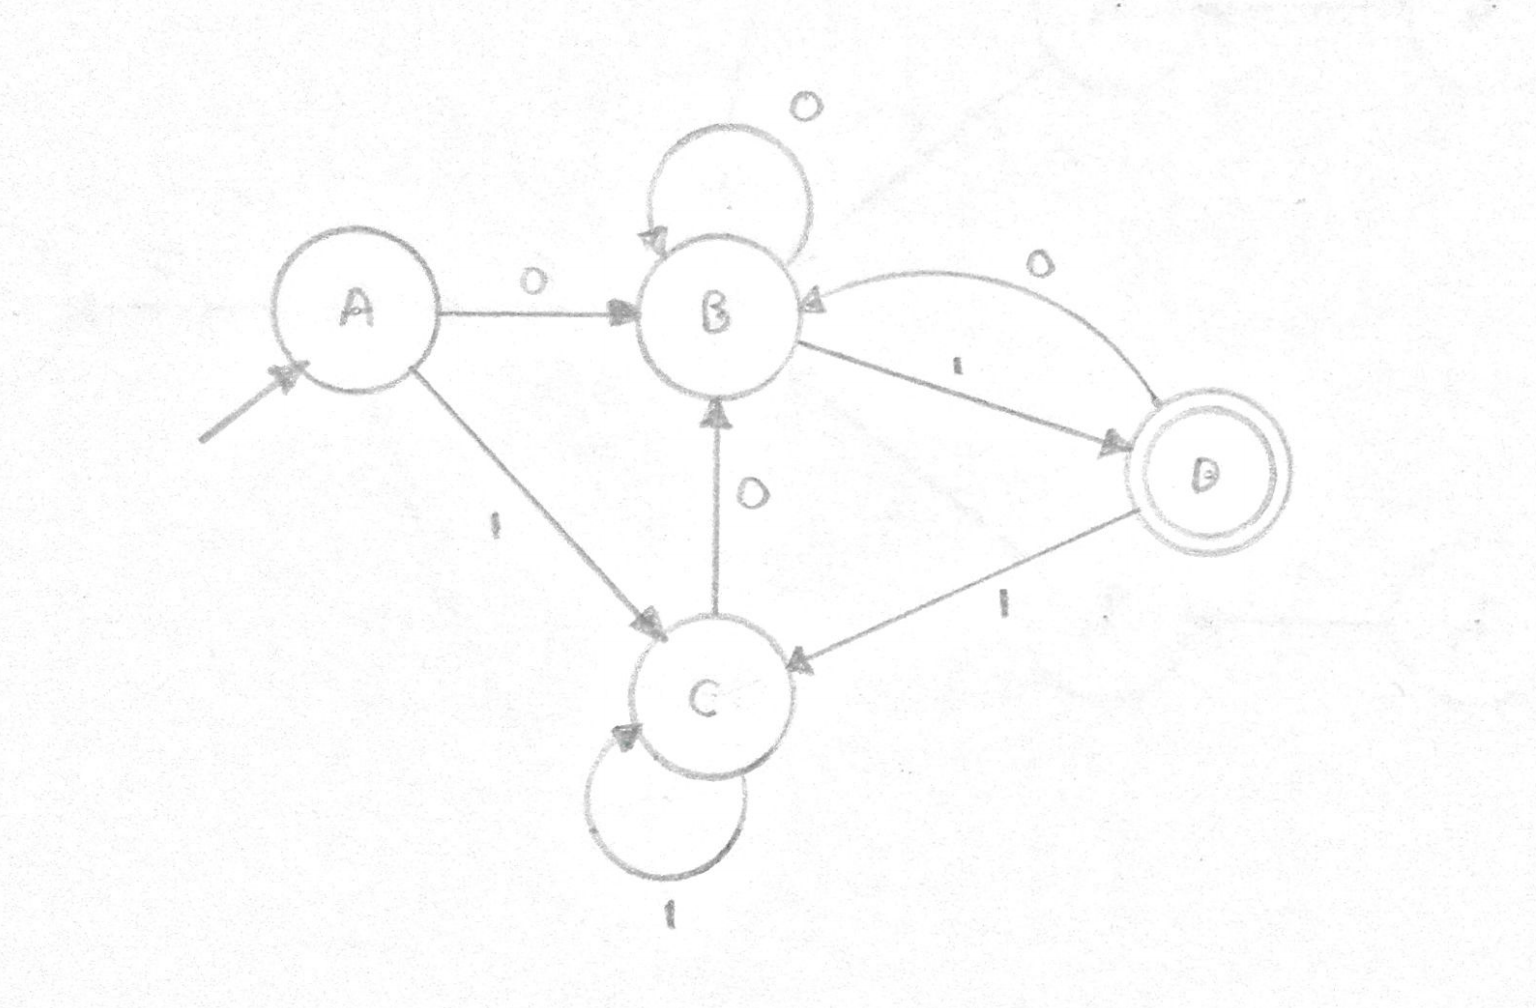
\includegraphics[width=\textwidth, height=9cm]{dfa}
\caption{El \textit{DFA} resultante de la tabla de estados.}
\end{figure}

\end{document}